\documentclass[a4paper, 11pt]{article}

\usepackage{fullpage} % Package to use full page
\usepackage{titling} % Title package
\usepackage{parskip} % Package to tweak paragraph skipping
\usepackage{tikz} % Package for drawing
\usepackage{amsmath}
\usepackage{multicol} % mutlicol management
\usepackage{hyperref} % for hyperlink and refs
\hypersetup{
    colorlinks = true,
    linkcolor = brown,
    linkbordercolor = {white},
}
\usepackage{caption} % for caption of pictures or table

% Language :
\usepackage[utf8]{inputenc}
\usepackage[english]{babel}
\usepackage[T1]{fontenc}
\usepackage{helvet}

% Symbols :
\usepackage{gensymb}

% Multi Column formating
\usepackage{multicol}
\setlength{\columnsep}{1cm}

% Algorithm :
\usepackage{algorithm}
\usepackage{algpseudocode}

%%%%%%%%% Pictures management : %%%%%%%%%
\usepackage{graphicx} % to insert png
\usepackage{adjustbox} % for better figure positionning
\usepackage[a4paper]{geometry} % for geometry changes in only one page (\newgeometry{...})
\usepackage[space]{grffile} % allow space in figure path
\usepackage{float}% Prevent pictures to moves to next page automatically

%%%%%%%%% Cosmetic Headers and footers : %%%%%%%%%
\usepackage{fancyhdr} % Custom headers and footers
\pagestyle{fancy} % Makes all pages in the document conform to the custom headers and footers
\fancyhead[R]{}
\fancyhead[L]{}
\fancyfoot[L]{} % Empty left footer
\fancyfoot[C]{} % Empty center footer
\fancyfoot[R]{\thepage} % Page numbering for right footer
\renewcommand{\headrulewidth}{0pt} % Remove header underlines
\renewcommand{\footrulewidth}{0pt} % Remove footer underlines
\setlength{\headheight}{13.6pt} % Customize the height of the header
\setlength{\footskip}{20pt} % Customize the skip of the footer
\setlength{\textheight}{650pt} % Customize the height of the text


%%%%%%%%% Personalized commands : %%%%%%%%%
\newcommand{\horrule}[1]{\rule{\linewidth}{#1}} % Create horizontal rule command with 1 argument of height



%--------------------------------------------------
%    TITLE SECTION
%-----------------------------Weightle---------------------
\pretitle{
  \begin{figure}[H] % floating picture
  \begin{center}
  
\includegraphics[width=0.80\textwidth]{../figures_trabalho_final/ufrj_logo.jpg}
\\[\bigskipamount]
}
\posttitle{
  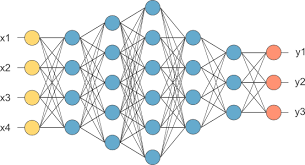
\includegraphics[width=0.65\textwidth]{../figures_trabalho_final/neural_network.png}
  \end{center} \end{figure}}

\title{
\normalfont \normalsize
%\textsc{Universidade Federal do Rio de Janeiro} \\ [25pt] % Your university, school and/or department name(s)
\horrule{0.5pt} \\[0.4cm] % Thin top horizontal rule
\huge \textbf{Energy consumption of buildings }\\
Classification according to their geometry\\ % The assignment title
\horrule{2pt} \\[0.5cm] % Thick bottom horizontal rule
}

\author{Guillaume Jeusel \\ \\
Palestra : NCG013 - Weigthless Neural Network \\ \\
Professor : Priscila Lima}

\date{\normalsize\today} % Today's date or a custom date


\begin{document}

\maketitle % Print the title
\newpage
\tableofcontents
\newpage

%------------------------------------------------------------------------------
\section{Introduction}

With an increasing energy demand worldwide, one of the majors problem of
our time is about energy consumption reduction. The concept of
\href{https://en.wikipedia.org/wiki/Negawatt_power}{NegaWatt}
traduces an energy-saving which originate from a change of behaviour
or a switch of technology used. And a domain in which a large amount of
progress can be done remains in the building consumption of energy.

Consequently, the research flourish in this area in order to
satisfy new directives and regulations for new building but also for olf
building renovation - (for example, the new
\href{https://ec.europa.eu/energy/sites/ener/files/documents/2010_mandate_480_en.pdf}
{210/31/EU} European directive).

Furthermore, using building energy simulation softwares may provide reliable solutions
to estimate the Energy Load. However this process can be very time-consuming
and requires user-expertise. Hence, in practice many researchers rely on
machine learning tools to study the effect of various building parameters
for the reasons it is easier and faster if a large enough database is
available.

In this study, we will focus on the classification of building's energy
consumption according to geometricals variables using
the
\href{https://www.elen.ucl.ac.be/Proceedings/esann/esannpdf/es2009-6.pdf}{WiSARD}
paradigm.

%------------------------------------------------------------------------------
\section{Presentation of the Dataset}

The Dataset comes from
\href{https://archive.ics.uci.edu/ml/datasets/Energy+efficiency}{UCI}
and is the results of 768 simulations using
\href{http://logiciels.i3er.org/ecotect.html}{Ecotect} software.
For each simulation, one of the geometrical input parameters was been
modified, which results in different Total Energy Load computed.
The variales are resumed in the following table :\medskip

\begin{center}
\begin{tabular}{llcc}
  \hline
  Var. & Var. meaning & N possible values & Unit \\
  \hline
  X1 & Relative Compactness & 12 & None \\
  X2 & Surface Area & 12 & $m^2$\\
  X3 & Wall Area & 7 & $m^2$\\
  X4 & Roof Area & 4 & $m^2$\\
  X5 & Overall Height & 2 & $m$\\
  X6 & Orientation & 4 & Unknown\\
  X7 & Glazing Area & 4 & $m^2$\\
  X8 & Glazing Area Distribution & 6 & None \\
  y & Total Load & 636 & Unknown \\
\end{tabular}\\
\captionof{table}{Input Variables and Output Variable}
\end{center}

From a previous work realized on this Dataset, X6 Orientation variable is
detected as decorrelated from every other input variables, and therefore
can be neglected safely.

\begin{figure}[H]
\begin{center}
  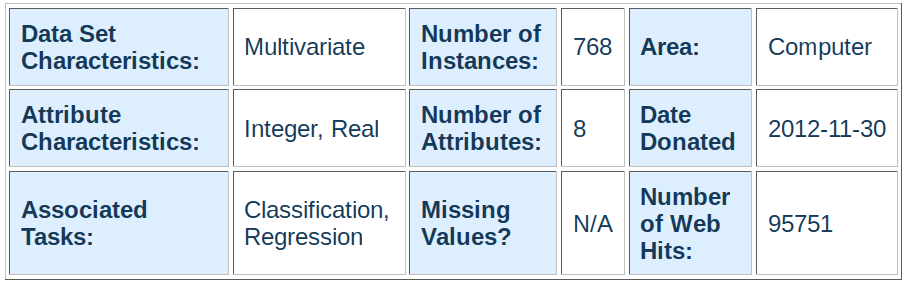
\includegraphics[scale=0.38]{../figures_trabalho_final/resume_dataset.png}
  \captionof{figure}{Other Characteristics}
\end{center}
\end{figure}

%------------------------------------------------------------------------------
\section{Dataset Formatting}

Initially, the \emph{energy-efficiency.csv} file is of the following form :
\begin{figure}[H]
\begin{center}
  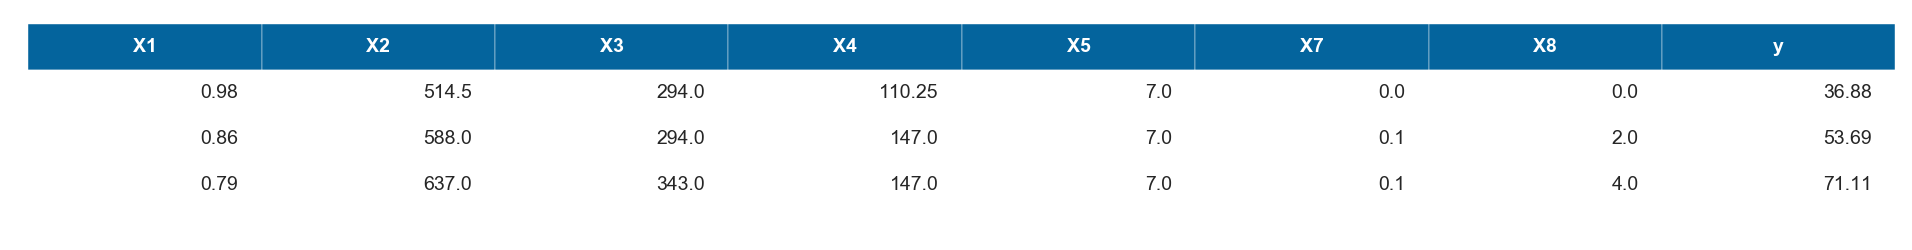
\includegraphics[width=\textwidth]{../figures_trabalho_final/step_df.png}
  \captionof{table}{Dataset after csv read}
\end{center}
\end{figure}

We will see in this section the steps leading to the dataset used for WiSARD
classifier.

%------------------------------------------------------------------------------
\subsection{Classification purpose}

\begin{multicols}{1}

\begin{wrapfigure}{l}{0.8\linewidth}
    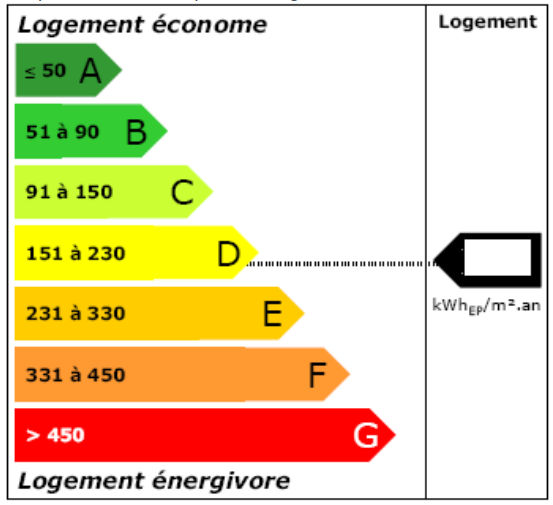
\includegraphics[width=0.95\linewidth]{../figures_trabalho_final/classification_consomation.png}
    \captionof{figure}{Example of Classification}
\end{wrapfigure}

We then transform this Dataset into a classification problem.
We will set a certain list of classes which isn't related to any official
classification, just for getting at least \textbf{4 classes} and a certain
level of complexity. (With only 2 classes, the accuracy was of 100\% with a
simple Gaussian Process Classifier.)
The choice made was the following :
\end{multicols}
\newpage

\begin{algorithm}
\begin{algorithmic}[1]
  \For {y $\in$ DataFrame['y Total Load']}
    \If {$y \in [0, 25[$}:
      \State $class \gets A$
    \ElsIf {$y \in [25, 50[$}:
      \State $class \gets B$
    \ElsIf {$y \in [50, 75[$}:
      \State $class \gets C$
    \ElsIf {$y \in [75, 100[$}:
      \State $class \gets D$
  \EndFor
\end{algorithmic}
\end{algorithm}

Which lead to the next form :
\begin{figure}[H]
\begin{center}
  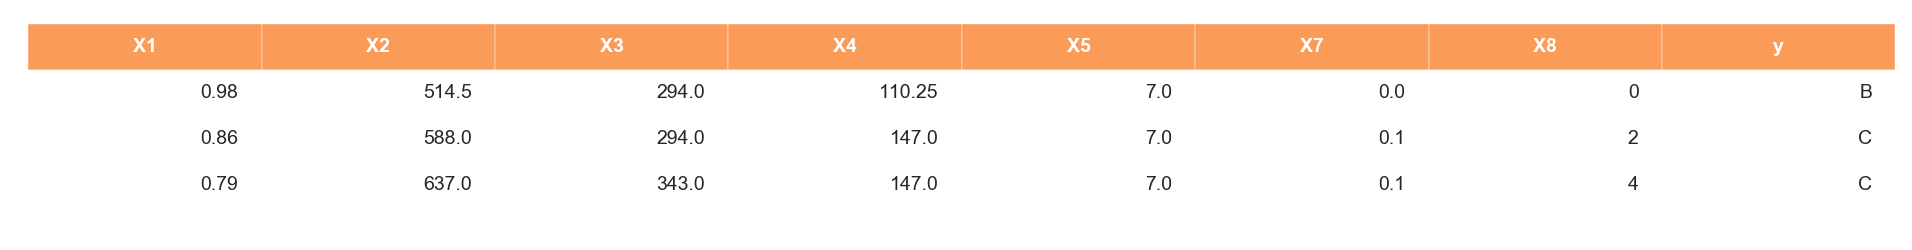
\includegraphics[width=\linewidth]{../figures_trabalho_final/step_df_classif.png}
  \captionof{table}{Dataset for Classification}
\end{center}
\end{figure}

%------------------------------------------------------------------------------
\subsection{Binarization}
The WiSARD model needs as entries only binaries.
So we will be using the \textbf{IEEE Standard for Floating-Point
Arithmetic} :
\begin{figure}[H]
\begin{center}
  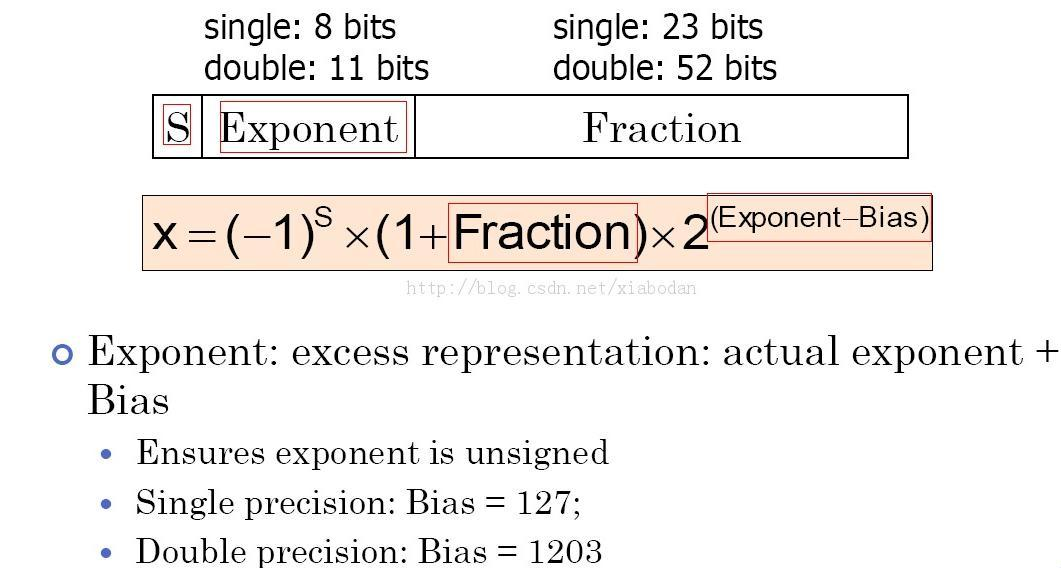
\includegraphics[width=0.8\linewidth]{../figures_trabalho_final/IEEE.jpg}
  \captionof{figure}{Explanation of IEEE binary representation of a float}
\end{center}
\end{figure}

Which finally will transform each float of the dataset into a list of binaries
representing this float as follow :
\begin{figure}[H]
\begin{center}
  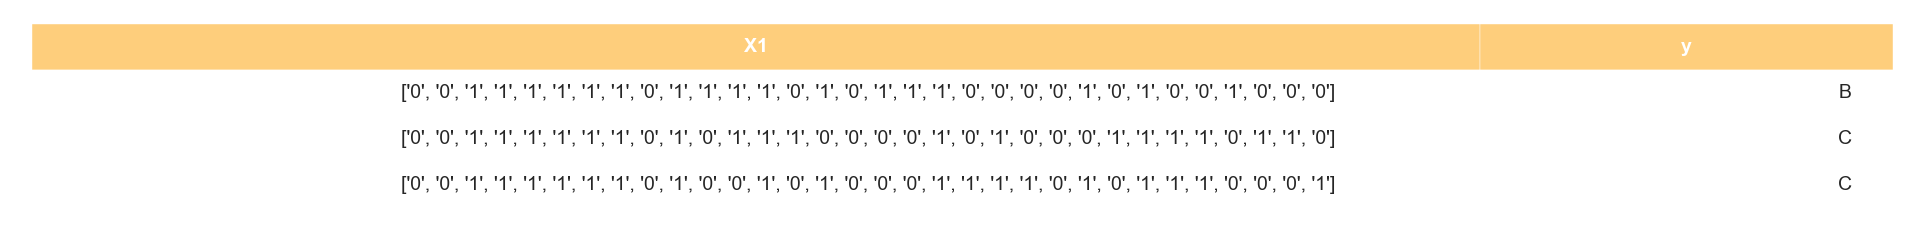
\includegraphics[width=\linewidth]{../figures_trabalho_final/step_df_bin_classif.png}
  \captionof{table}{Dataset Binarized, showing only X1}
\end{center}
\end{figure}


%------------------------------------------------------------------------------
\section{Results}
Due to a lack of registers in the dataset, the use of cross-validation
with randomly choosen train and test sets where required for validation sake.

\begin{itemize}
   \item For WiSARD parameters calibration : only 20 folds with $90\%$ for
     the training set and $10\%$ for the test set.
   \item For \textbf{overall} scores : 40 folds with $90\%$ for
     the training set and $10\%$ for the test set.
    \item The \textbf{accuracy} is then computed as the mean of all accuracies obtained
      over the folds.
\end{itemize}

%------------------------------------------------------------------------------
\subsection{WiSARD parameters calibration}

We will study the influence of the \textbf{num\_bits\_addr} and the
\textbf{bleaching} variables.

The following graphic shows the \textbf{accuracy} according to this variables :
\begin{figure}[H]
\begin{center}
  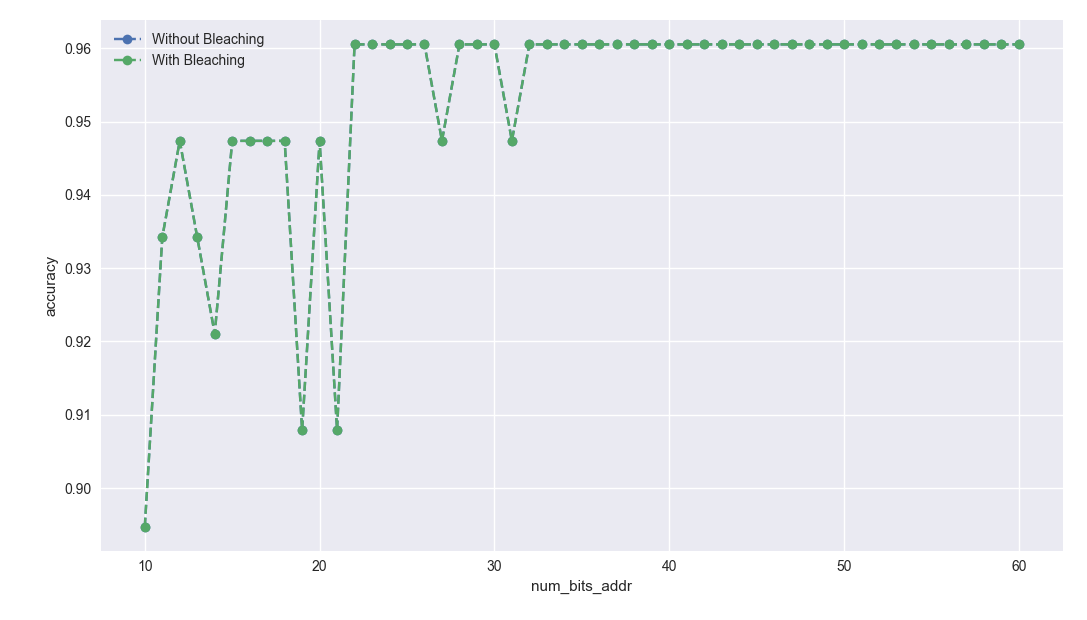
\includegraphics[width=\linewidth]{../figures_trabalho_final/wisard_parameters_results.png}
  \captionof{figure}{WiSARD Accuracy}
\end{center}
\end{figure}

It appears that there is no influence using or not the
bleaching method, and that for more than \textbf{32 num\_bits\_addr} there is no
improvement on the accuracy. This number correspond to the chosen precision of
float representation.


%------------------------------------------------------------------------------
\subsection{Overall Scores}

Comparing to others classifications methods with 40 folds used for
cross-validation :
\begin{figure}[H]
\begin{center}
  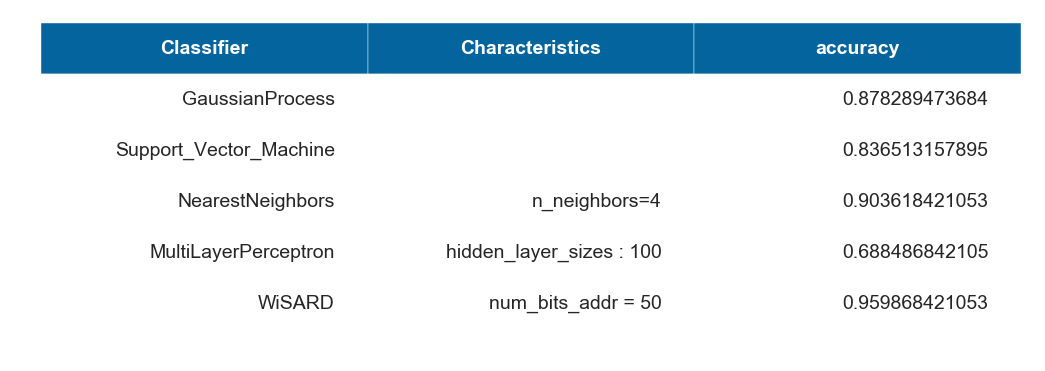
\includegraphics[width=\linewidth]{../figures_trabalho_final/overall_results.png}
  \captionof{table}{Comparing scores}
\end{center}
\end{figure}

And WiSARD clasification gives pretty good results !


%------------------------------------------------------------------------------
\section{Outlooks}

\begin{itemize}
  \item Change the representation of the floats into a \emph{thermomether}-like
    binary representation.
  \item Try to use the WiSARD for regression purpose.
\end{itemize}

GitHub python code adress : \url{https://github.com/gjeusel/NCG013_redes_neurais_sem_peso}











\end{document}
